\documentclass{article}   	% use "amsart" instead of "article" for AMSLaTeX format
\usepackage{geometry}                		% See geometry.pdf to learn the layout options. There are lots.
\geometry{letterpaper}                   		% ... or a4paper or a5paper or ... 
\usepackage{graphicx}				% Use pdf, png, jpg, or eps§ with pdflatex; use eps in DVI mode
\usepackage{amsmath}
\usepackage{amssymb}
\usepackage{natbib}
\usepackage{lineno}
\usepackage{color}
\usepackage{hyperref}
\linenumbers


\title{DESI Observations of Type Ia Supernovae Discovered by Imaging Surveys}


\begin{document}
\maketitle

\section{Host Redshifts of ZTF Discoveries with Good Light Curves}
ZTF will discover SNe~Ia that ultimately get ``good'' light curve measurements.  ZTF is expected to have discovery completeness to $z=0.15$.
For an imagined survey that overlaps ZTF and DESI fields, Nordin has estimated the
numbers of SN~Ia discoveries, the numbers of those with good light curves, and the numbers with redshifts from the SED~Machine.
The estimates are shown in Figure~\ref{ZTFnum:fig}.  (I presume some SNe with redshifts don't have good light curves.) 
The DESI footprint
is 14,000 square degrees.  Assuming that the 961 supernovae with good light curves are distributed uniformly, there will be 0.069
of these per square degree, or 0.5 per instrumented DESI footprint.


\begin{figure}[h]
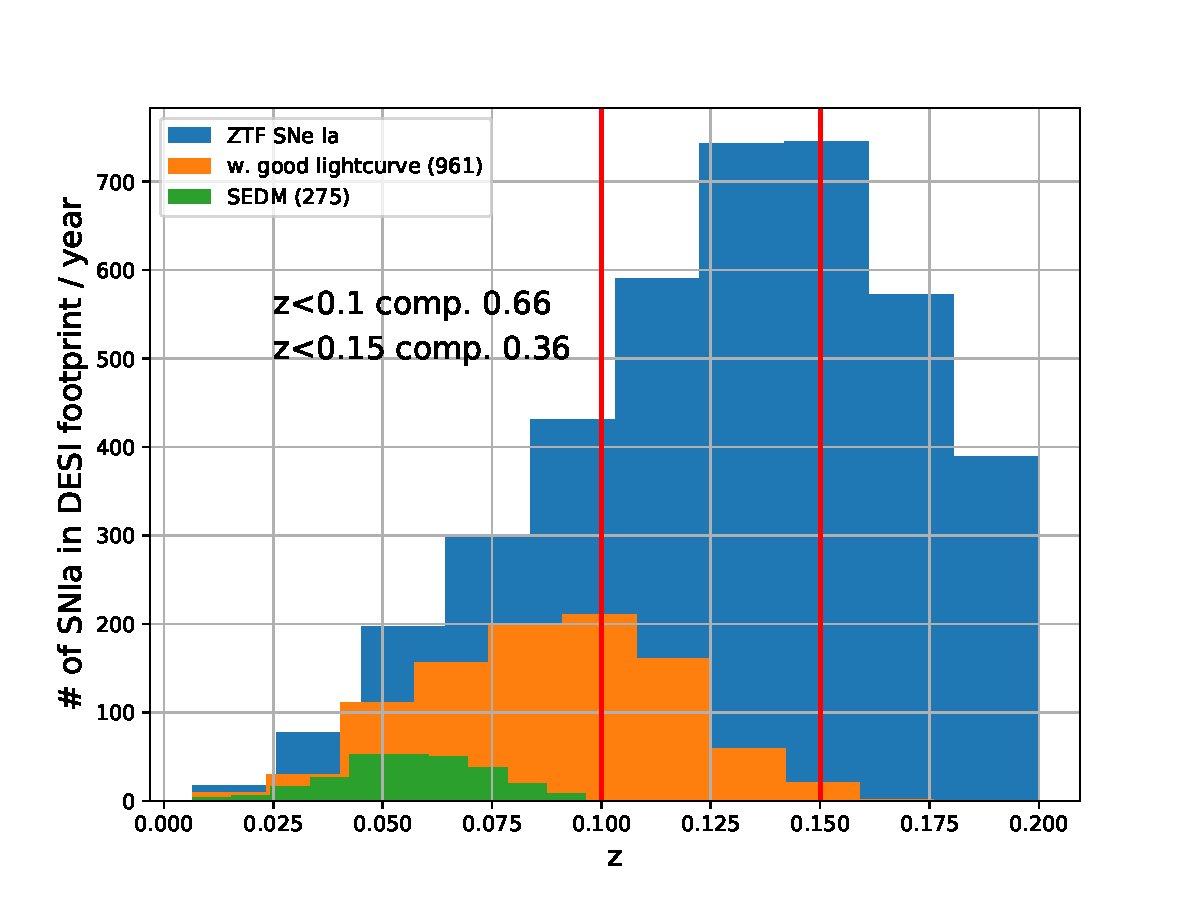
\includegraphics[width=8cm]{zdist_12m_185_195.pdf}
\centering
\caption{Numbers of ZTF SN~Ia discoveries, the numbers of those with good light curves, and the numbers with redshifts from the SED~Machine.
\label{ZTFnum:fig}}
\end{figure}

Redshifts of the host galaxies will be obtained using the SED~Machine, serendipitously as a DESI Bright Galaxy Survey (or other) target.
More redshifts could be obtained using spare fibers available during the DESI survey.

A rough estimate (calculated
using mock.py)
of the fraction of supernovae in a DESI BGS field 
that occur in a host galaxy with a successful DESI redshift is shown in Figure~\ref{19.5:fig}.
At redshift $z=0.15$, where ZTF is complete and the upper-redshift limit for objects with good light curves, half of ZTF supernovae will have a DESI redshift.
At redshift $z=0.1$, where the distribution of supernovae with good light curves peaks, 70\% of ZTF supernovae will have a DESI redshift.
That fraction increases to near-completeness as redshift decreases to zero.
The vast majority of missing redshifts are
because the host galaxy is too faint to be targeted in the BGS survey.
The remaining effects are
a 97 (92)\% efficiency for fiber allocation and a 92 (77)\% efficiency of extracting a redshift from the data for Tier 1(2) targets. 

\begin{figure}[h]
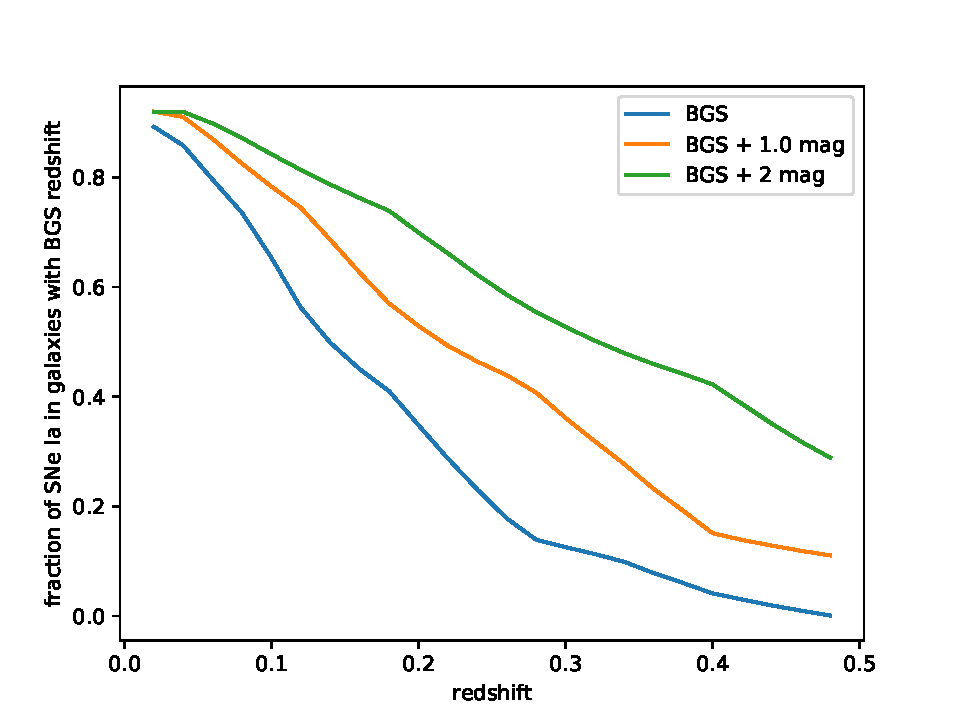
\includegraphics[width=8cm]{bg_frac.pdf}
\centering
\caption{Fraction of supernovae in a DESI BGS field 
that occur in a host galaxy with a successful DESI redshift.  Also shown are the fraction of supernovae that would occur in a host galaxy
with a successful DESI redshift (assuming 100\% fiber-allocation efficiency) shifting the efficiencies 1 and 2 mag deeper than the nominal BGS exposure.
\label{19.5:fig}}
\end{figure}

A candidate program to obtain redshifts of hosts not obtained by the BGS is to target host galaxies down to a fainter magnitude limit.
Figure~\ref{19.5:fig} shows the fractions of supernovae that would occur in a host galaxy
with a successful DESI redshift (now assuming 100\% fiber-allocation efficiency) shifting the efficiencies 1 and 2 mag deeper than the nominal BGS exposure.
(I believe that the standard DESI survey is 2-mag deeper than the BGS.)
At redshift $z=0.15$,  $\sim 80$\% of ZTF supernovae could get a DESI redshift going 2-magnitudes deeper than BGS.
At redshift $z=0.1$, 90\% of ZTF supernovae will have a DESI redshift.


Summary: Over the course of its survey, ZTF will discover $\sim 960$ SNe~Ia with good light curves.  With a matched field of view,
the DESI BGS survey will ``automatically'' obtain redshifts of a fraction of the brightest galaxies in the field, so that a significant majority
of supernovae with good light curves will have a redshift.   By targeting supernova host galaxies down to a fainter limiting magnitude,
DESI could increase the number of host-galaxy redshifts be a factor $\sim 2$ at the extreme redshift of $z=0.15$.  The number of targets would be
$\ll 0.25$ per DESI footprint.

\section{Active Type Ia Supernovae}
DESI can detect and/or classify active SNe~Ia in its spectra.  The spectrum could be of a primary DESI target, or a secondary target 
of a transient discovered elsewhere, presumably an imaging survey that is more efficient at discovery.

Shown in Figure~\ref{cum:fig} are cumulative number densities as a function of redshift of SNe~Ia instantaneously brighter than several $r$ limiting magnitudes. 
The result is a product of supernova rates, differential volumes, and control times.

\begin{figure}[h]
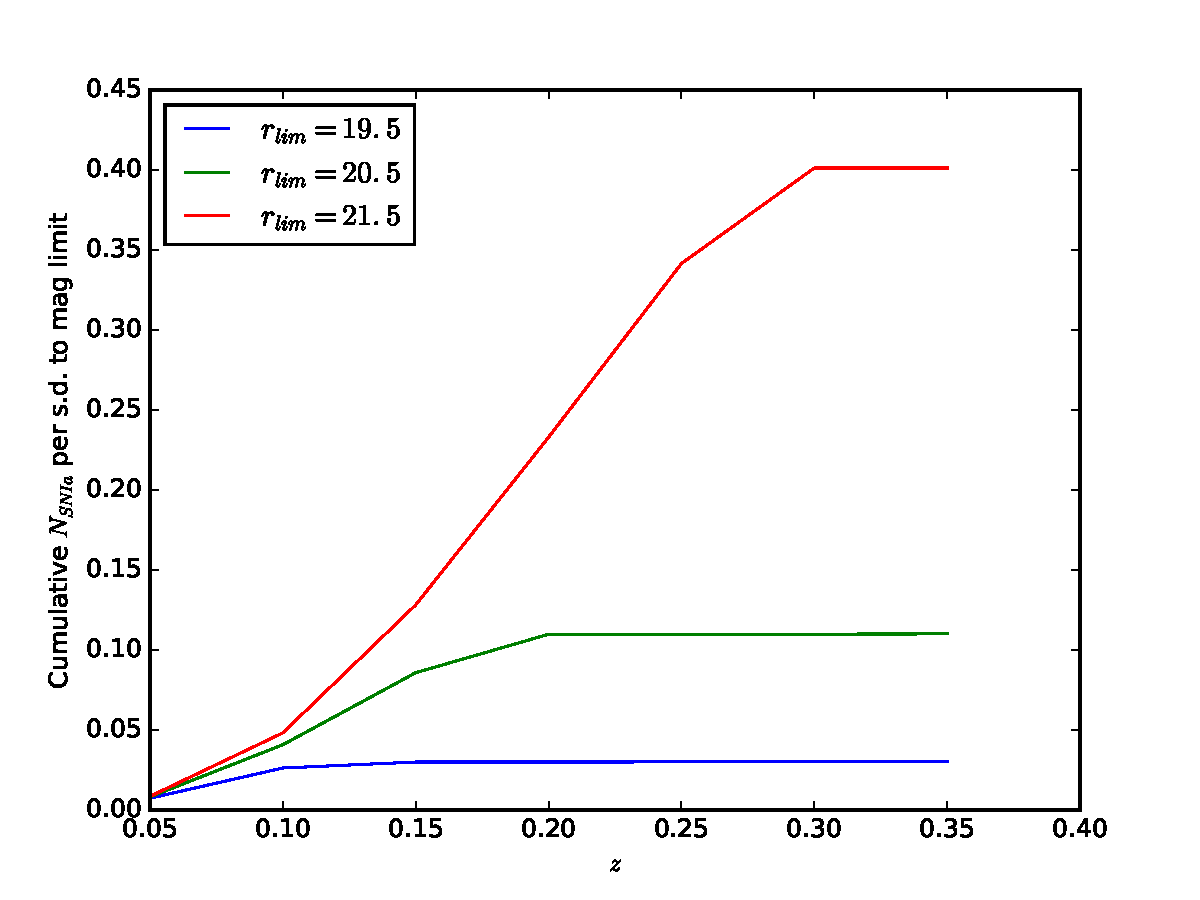
\includegraphics[width=8cm]{../src/cumulative.pdf}
\centering
\caption{Cumulative number densities as a function of redshift of SNe~Ia instantaneously brighter than several $r$ limiting magnitudes
\label{cum:fig}}
\end{figure}


\end{document} 
